\documentclass[letterpaper]{article}
\usepackage{spconf,amsmath,amssymb,graphicx}
\usepackage{hyperref}

\title{Efficient Parallelization of Bor\r{u}vka's Minimum Spanning Tree Algorithm}

\fiveauthors
  {Samuel Anzalone \\[-0.8ex] {\small BS Computational Science} \\[-0.8ex] {\small \texttt{ansamuel@ethz.ch}}}
  {Mike Marti \\[-0.8ex] {\small MS Computer Science} \\[-0.8ex] {\small \texttt{mikmarti@ethz.ch}}}
  {Matteo Kamm \\[-0.8ex] {\small MS Computer Science} \\[-0.8ex] {\small \texttt{matkamm@ethz.ch}}}
  {Hulda L.\ Hannesdóttir \\[-0.8ex] {\small MS Computer Science} \\[-0.8ex] {\small \texttt{hhannesdo@ethz.ch}}}
  {\v{S}imon Hrabec \\[-0.8ex] {\small MS Computer Science} \\[-0.8ex] {\small \texttt{shrabec@ethz.ch}}}

\begin{document}

\maketitle

\begin{abstract}
% Describe in concise words what you do, why you do it (not necessarily
% in this order), and the main result.  The abstract has to be
% self-contained and readable for a person in the general area. You
% should write the abstract last.
\end{abstract}

\section{Introduction}
\label{sec:intro}
In this section we briefly introduce and explain what Minimum-Spanning-Tree algorithms are used for. In addition, we
describe our contribution to the scientific comunity as well as work related to ours.

\mypar{Motivation}
Minimum-Spanning-Tree (MST) algorithms take weighted graphs as inputs and return spanning trees with minimal edge weight sums.

The MST problem is one of the most studied problems in combinatorial optimization \cite{graham1985history}. Although the
problem is rather simple, its solutions are often used as part of other algorithms to compute intermediate results. 
Other scientific fields, such as epidemiology or taxonomy, apply MST algorithms. Examples of problems that can be solved
using MST algorithms include
\begin{itemize}
  \item \textbf{Networking} MST algorithms find solutions for the Spanning Tree Protocol, which
    is used to avoid bridge loops for Ethernet networks. % TODO: Does STP actually use MST?
  \item \textbf{$\frac{3}{2}$-ap\-prox\-i\-mate metric TSP} By combining algorithms that find MSTs, matchings and
    eulerian circuits, one can develop a $\frac{3}{2}$-ap\-prox\-i\-mation algorithm solving the metric traveling
    salesperson problem \cite{christofides1976worst}.
  \item \textbf{Molecular Epidemiology} Minimum-Spanning-Trees are used in molecular epidemiology research to estimate
    relationships among individual strains or isolates \cite{spada2004use, salipante2011inadequacies}.
  \item \textbf{Machine Learning} MSTs are used as part of machine learning algorithms. For example, MSTs reduce the
    fraction of incorrectly labeled samples when performing brain MRI tissue classification \cite{cocosco2003fully}.
\end{itemize}
For most of these use cases, the speed of the MST algorithm is of great importance e.g. to get quick medical results and
be able to treat the patient accordingly.

\mypar{Contribution}
In our research, we focused on the MST algorithm proposed by Bor\r{u}vka \cite{boruuvka1926jistem,
nevsetvril2001otakar}, which is one of the most prominent MST algorithms as of today. We implemented this algorithm
using different work distribution strategies. Our implementations use the Message Passing Interface
(MPI) for work distribution and communication. To evaluate the performance of our implementations, we use
randomly generated Kronecker graphs.

\mypar{Related Work}
% TODO maybe find more references for the first paragraph
As the MST problem is very versatile and can be used in various scientific disciplines, there already is some research
on parallelizing MST algorithms. One such paper \cite{chung1996parallel}, which is also the main inspriation of this
project, evaluates how the performance of Bor\r{u}vka behaves when using different pointer jumping schemes.

Other research focuses on the difference in performance with regards to the computation model \cite{dehne1998practical}.
Furthermore, other research focuses on the parallelization  of the MST algorithm using GPUs \cite{de2017parallel}.

Our research is similar to that of Chung and Condon \cite{chung1996parallel}, but differs in that we also look at
different work distribution strategies. % TODO: Move this to the first paragraph of related work?

% TODO: Mention this related work: https://citeseerx.ist.psu.edu/viewdoc/download?doi=10.1.1.5.9759&rep=rep1&type=pdf

% TODO remove
% Do not start the introduction with the abstract or a slightly modified
% version. It follows a possible structure of the introduction. 
% Note that the structure can be modified, but the
% content should be the same. Introduction and abstract should fill at most the first page, better less.
%
% \mypar{Motivation} The first task is to motivate what you do.  You can
% start general and zoom in one the specific problem you consider.  In
% the process you should have explained to the reader: what you are doing,
% why you are doing, why it is important (order is usually reversed).
%
% For example, if my result is the fastest sorting implementation ever, one
% could roughly go as follows. First explain why sorting is important
% (used everywhere with a few examples) and why performance matters (large datasets,
% realtime). Then explain that fast implementations are very hard and
% expensive to get (memory hierarchy, vector, parallel). 
%
% Now you state what you do in this paper. In our example: 
% presenting a sorting implementation that is
% faster for some sizes as all the other ones.
%
% \mypar{Related work} Next, you have to give a brief overview of
% related work. For a report like this, anywhere between 2 and 8
% references. Briefly explain what they do. In the end contrast to what
% you do to make now precisely clear what your contribution is.

\section{Background}
\label{sec:background}
In this section we will introduce the MST problem itself, as well as Bor\r{u}vka's algorithm and different
parallelization strategies used in our implementations.

\mypar{Spanning Tree/Forest}
TODO

\mypar{Minimum-Spanning-Tree Problem}
TODO

\mypar{Bor\r{u}vka's Algorithm}
TODO

\mypar{Union Find Datastructure}
TODO

\mypar{Pointer Jumping}
TODO

\mypar{Supervertex Pointer Jumping}
TODO

\mypar{MPI}
TODO

\mypar{Kronecker Graphs}
% TODO Not sure if this is the original paper that introduced kronecker graphs (double check)
TODO \cite{leskovec2010kronecker}

% Give a short, self-contained summary of necessary
% background information. For example, assume you present an
% implementation of sorting algorithms. You could organize into sorting
% definition, algorithms considered, and asymptotic runtime statements. The goal of the
% background section is to make the paper self-contained for an audience
% as large as possible. As in every section
% you start with a very brief overview of the section. Here it could be as follows: In this section 
% we formally define the sorting problem we consider and introduce the algorithms we use
% including a cost analysis.
%
% \mypar{Sorting}
% Precisely define sorting problem you consider.
%
% \mypar{Sorting algorithms}
% Explain the algorithm you use including their costs.
%
% As an aside, don't talk about "the complexity of the algorithm.'' It's incorrect,
% problems have a complexity, not algorithms.


\section{Approach}
\label{sec:approach}

Now comes the ``beef'' of the report, where you explain what you
did. Again, organize it in paragraphs with titles. As in every section
you start with a very brief overview of the section.

In this section, structure is very important so one can follow the technical content.

Mention and cite any external resources that you used including libraries or other code.

\section{Experimental Results}\label{sec:exp}

Here you evaluate your work using experiments. You start again with a
very short summary of the section. The typical structure follows.

\mypar{Experimental setup} Specify the platform (processor, frequency, maybe OS, maybe cache sizes)
as well as the compiler, version, and flags used. If your work is about performance, 
I strongly recommend that you play with optimization flags and consider also icc for additional potential speedup.

Then explain what kind of benchmarks you ran. The idea is to give enough information so the experiments are reproducible by somebody else on his or her code.
For sorting you would talk about the input sizes. For a tool that performs NUMA optimization, you would specify the programs you ran.

\mypar{Results}
% TODO compare to results from Chung and Condon
Next divide the experiments into classes, one paragraph for each. In each class of experiments you typically pursue one questions that then is answered by a suitable plot or plots. For example, first you may want to investigate the performance behavior with changing input size, then how your code compares to external benchmarks.

For some tips on benchmarking including how to create a decent viewgraph see pages 22--27 in \cite{Pueschel:10}.

{\bf Comments:}
\begin{itemize}
\item Create very readable, attractive plots (do 1 column, not 2 column plots
for this report) with readable font size. However, the font size should also not be too large; typically it is smaller than the text font size.
An example is in Fig.~\ref{fftperf} (of course you can have a different style).
\item Every plot answers a question. You state this question and extract the
answer from the plot in its discussion.
\item Every plot should be referenced and discussed.
\end{itemize}

\begin{figure}\centering
  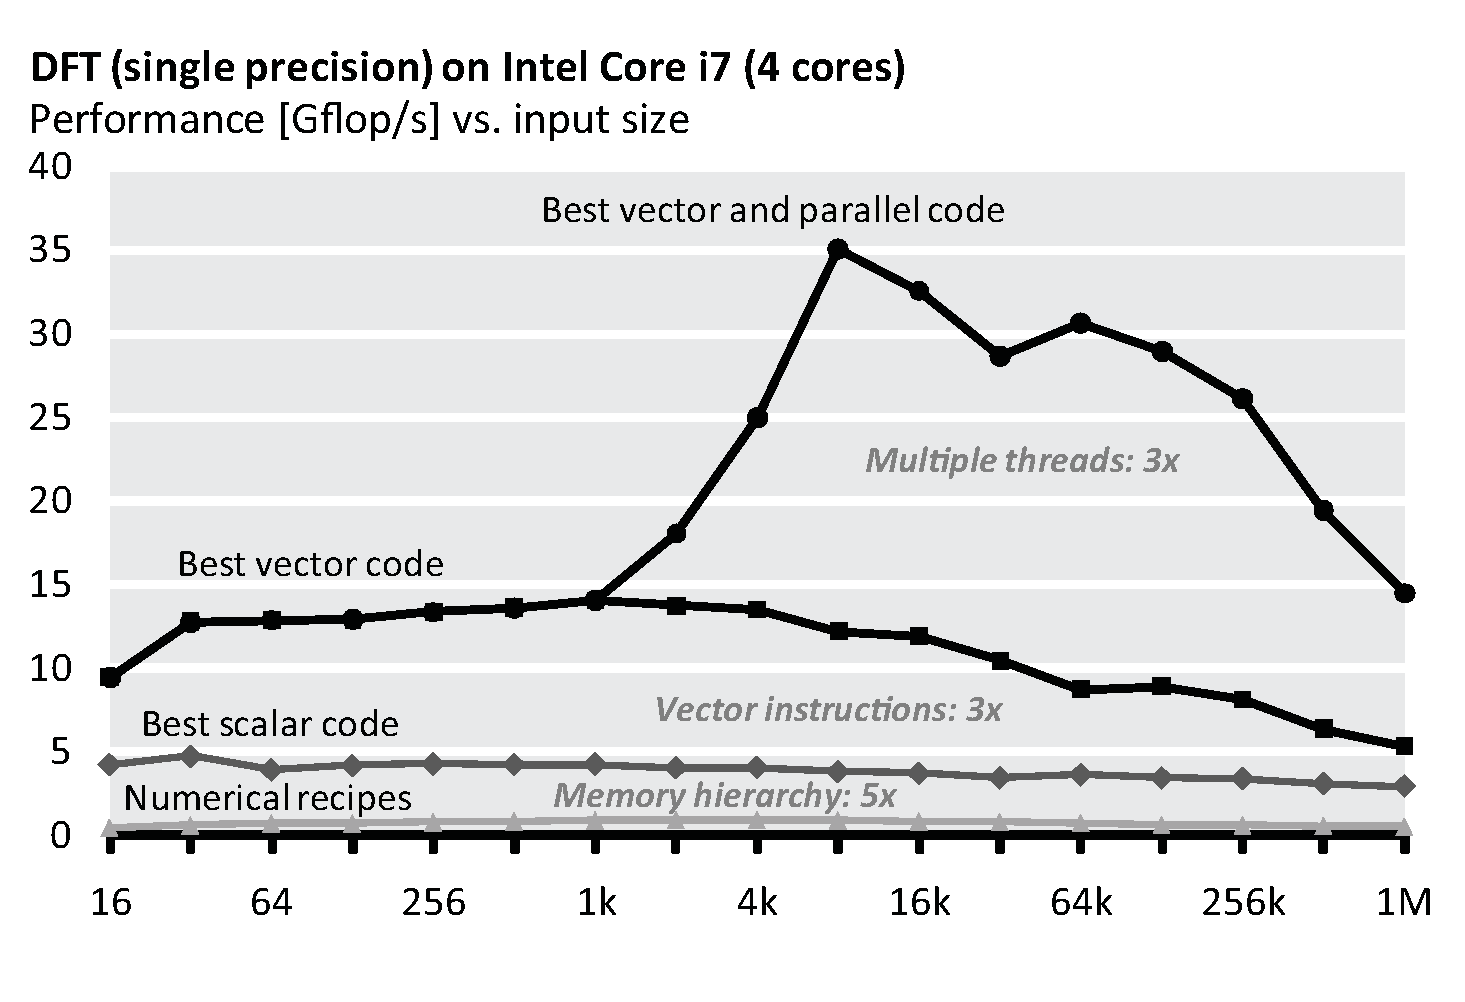
\includegraphics[scale=0.33]{dft-performance.eps}
  \caption{Performance of four single precision implementations of the
  discrete Fourier transform. The operations count is roughly the
  same. The labels in this plot are maybe a little bit too small.\label{fftperf}}
\end{figure}

\section{Conclusions}

Here you need to summarize what you did and why this is
important. {\em Do not take the abstract} and put it in the past
tense. Remember, now the reader has (hopefully) read the report, so it
is a very different situation from the abstract. Try to highlight
important results and say the things you really want to get across
such as high-level statements (e.g., we believe that .... is the right
approach to .... Even though we only considered x, the
.... technique should be applicable ....) You can also formulate next
steps if you want. Be brief. After the conclusions there are only the references.

\section{Further comments}

Here we provide some further tips.

\mypar{Further general guidelines}

\begin{itemize}
\item For short papers, to save space, I use paragraph titles instead of
subsections, as shown in the introduction.

\item It is generally a good idea to break sections into such smaller
units for readability and since it helps you to (visually) structure the story.

\item The above section titles should be adapted to more precisely
reflect what you do.

\item Each section should be started with a very
short summary of what the reader can expect in this section. Nothing
more awkward as when the story starts and one does not know what the
direction is or the goal.

\item Make sure you define every acronym you use, no matter how
convinced you are the reader knows it.

\item Always spell-check before you submit (to us in this case).

\item Be picky. When writing a paper you should always strive for very
high quality. Many people may read it and the quality makes a big difference.
In this class, the quality is part of the grade.

\item Books helping you to write better: \cite{Higham:98} and \cite{Strunk:00}.

\item Conversion to pdf (latex users only): 

dvips -o conference.ps -t letter -Ppdf -G0 conference.dvi

and then

ps2pdf conference.ps
\end{itemize}

\mypar{Graphics} For plots that are not images {\em never} generate the bitmap formats
jpeg, gif, bmp, tif. Use eps, which means encapsulate postscript. It is
scalable since it is a vector graphic description of your graph. E.g.,
from Matlab, you can export to eps.

The format pdf is also fine for plots (you need pdflatex then), but only if the plot was never before in the format 
jpeg, gif, bmp, tif.

\bibliographystyle{IEEEbib}
\bibliography{bibl_conf}

\end{document}

